\chapter{概览}
\label{cap:overview}
    我们设计的性能预测工具,目标是预测深度神经网络在特定平台上的运行时间。主要工作分为操作性能建模和调度模拟两部分。本章将详细介绍我们设计的预测系统。
    
\section{系统配置}
    系统的输入分为两部分,待预测的深度神经网络模型和运行的硬件平台参数。
    
    其中,带预测模型的输入不仅需要提供计算的定义,还需要提供输入数据的规模参数。定义网络的时候,通常不需要在模型定义的时候严格限定输入的规模。批量大小(Batch-size)通常也是训练过程中需要调整的一个重要参数。如图\ref{fig:dag_same}所示,在这种情况下,输入规模的变化并不会影响数据流图的生成。因此,用户在使用性能预测工具的时候,还需要额外输入数据规模的相关参数。

    此外我们的系统中所有性能数据都需要保证是当前选择平台的实测数据。因此目前只提供数量有限的配置选择。用户在进行预测时自行选择。

    \begin{figure}[!htbp]
        \centering
        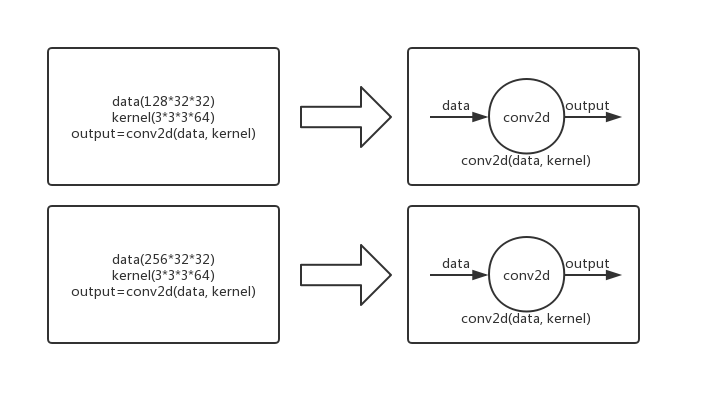
\includegraphics[width=0.8\textwidth]{figures/dag_same.jpg}
        \caption{模型相同,输入规模不同,数据流图相同}
        \label{fig:dag_same}
    \end{figure}
    
    
\section{系统架构}
    我们的预测系统整体架构如图\ref{fig:arch}所示。我们的实现主要分为两部分,即途中的性能模型和调度模拟。
    
    性能模型部分,我们选定三个在一般卷积神经网络中占用时间最长的操作,对每个操作的运行时间进行单独的性能分析,建立性能模型。
    
    调度模拟部分,我们根据用户输入的模型定义,构造数据流图。按照TensorFlow的运行过程,对图进行预处理。之后根据TensorFlow的执行策略模拟运算的调度过程,得到模型的整体运行时间。

    \begin{figure}[!htbp]
        \centering
        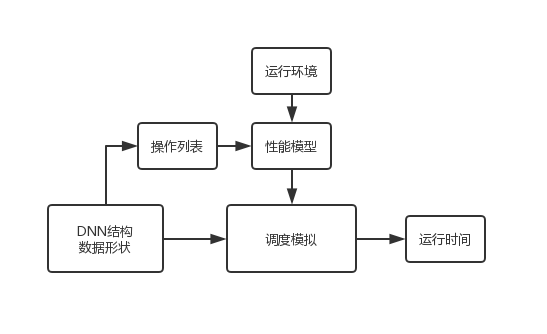
\includegraphics[width=0.8\textwidth]{figures/arch.jpg}
        \caption{整体架构}
        \label{fig:arch}
    \end{figure}


\section{性能模型}
    在卷积神经网络中,模型的结构通常是分层的。主要包含三类:卷积层、池化层、全连接层。在实际的使用中,层间可能会根据模型需要加入归一化、Dropout等层。而TensorFlow支持的操作总数较多,我们对所有操作均建立性能模型是不现实的,因此我们需要选择合适的操作,进行性能建模。
    
    AlexNet\cite{alexnet}是一个典型的卷积神经网络。我们以AlexNet在CPU上执行的时间轴数据为例,如图\ref{fig:alexnet_timeline}所示。我们可以观察到,二维卷积(包括正向和反向)、矩阵乘法、归一化(包括反向)三个操作贡献了几乎所有的运行时间。事实上,这三个操作在运行过程中占用了运行时间的95\%以上。因此,我们只需要对这三个操作进行建模,就可以很好地服务卷积神经网络了。
    
    特别地,图\ref{fig:alexnet_timeline}中占用时间较多的局部相应归一化(LRN)函数以及其梯度函数(LRNGrad)是AlexNet中特有的层,在目前最先进的工作中,使用已经较少。我们为了验证我们的系统合理性,依旧对其进行建模,而针对大部分卷积神经网络,二维卷积和矩阵乘法已经可以足够预测的使用了。

    \begin{figure}[!htbp]
        \centering
        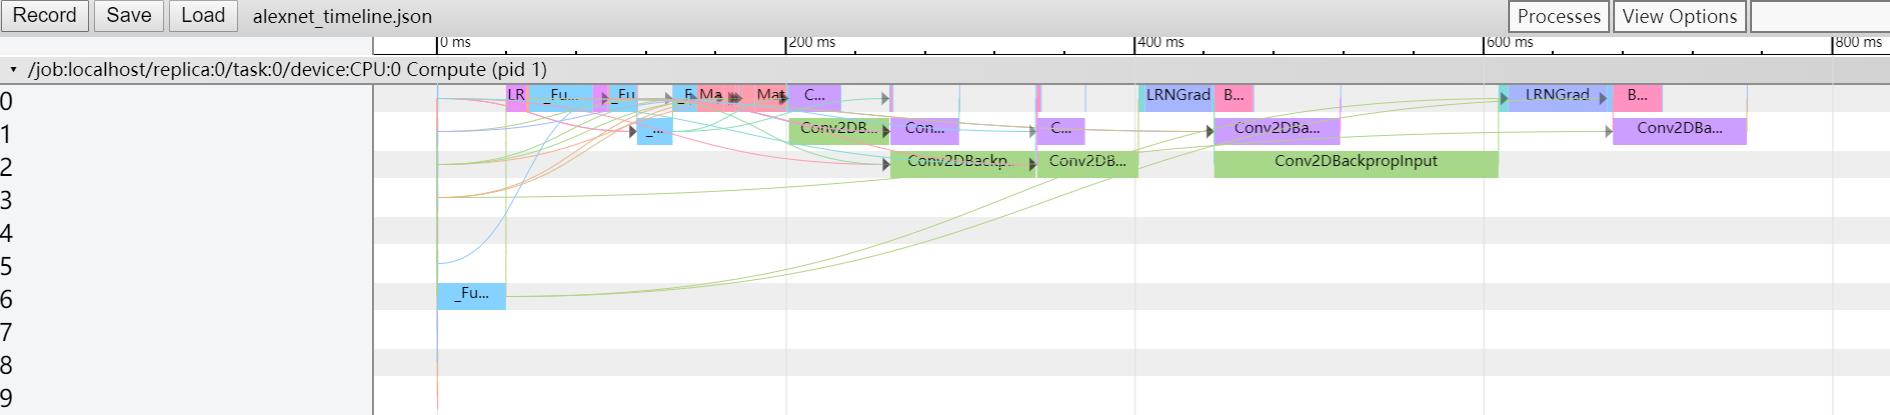
\includegraphics[width=0.8\textwidth]{figures/alexnet_timeline.png}
        \caption{AlexNet在CPU执行的时间轴数据}
        \label{fig:alexnet_timeline}
    \end{figure}


\subsection{矩阵乘法}
\label{ssec:view_matmul}
    全连接层是卷积神经网络中非常重要的组成部分,通常出现在卷积神经网络的最后基层,将卷积层得到的局部特征进行综合。全连接层的操作就是二维矩阵的乘法。相比其他操作,全连接层的参数数大,运行时间长。因此,对矩阵乘法进行性能建模时非常有必要的。
    
    矩阵乘法的输入为两个矩阵,即两个二维张量。其中矩阵$ A $的形状为$ M \times P $,矩阵$ B $的形状为$ P \times N $,输出为矩阵$ C = A \times B $,形状为$M \times N$。其中,$ C_{m, n} = \sum_{p=1}^P{a_{m, p} \times b_{p, n}} $。
    
    在单线程运行情况下,矩阵乘法的复杂度为$ O(M N P) $。然而,由于数据的局部性,即使$ M \times N \times P $固定,将两个参数交换,如交换$ N $和$ P $,矩阵乘法操作的运行时间是不同的。我们在建模的时候不能仅仅选取$ M \times N \times P $作为参数。
    
    在CPU多线程计算或使用GPU计算的情况下,一般会对矩阵乘法运算进行展开。这种情况下任务会被转化为$ M \times N $个$ P $维向量点积,因此在较大规模的情况下,我们可以合并$ M $和$ N $,用来提高预测精度。这一部分将会在\ref{ssec:impl_matmul}节进行详细讨论。

    在TensorFlow中,系统会根据运算的规模和使用的硬件平台,讲矩阵乘法映射到不同的函数。以CPU为例,数据规模较小的时候,TensorFlow会直接进行计算,而数据规模较大的时候系统可能会调用Eigen\cite{eigen}中的函数。在GPU中,系统会根据规模的不同选用不同的CuBlas函数进行计算,我们的性能预测模型需要针对这一性质有所考虑。

    此外,矩阵乘法的梯度求解依然是矩阵乘法。在TensorFlow中,矩阵乘法的梯度求解并没有作为一个单独的操作出现,因此我们不需要考虑矩阵乘法的梯度函数建模问题。


\subsection{二维卷积}
\label{ssec:view_conv}
    二维卷积是卷积神经网络的核心运算,占用了卷积神经网络中最多的运算时间。通常来说,卷积层和池化层是成对出现的。卷积层通过二维卷积运算提取局部特征,池化层通过选取局部最大这类操作减少参数规模。由于池化操作并不包含运算,因此在TensorFlow中,二维卷积和池化操作是合并进行的。因此,我们只需要测试二维卷积的运行时间,就可以很好地预测卷积层和池化层的运行时间了。

    在TensorFlow中使用二维卷积操作,需要三个张量作为输入:输入数据、卷积核、步长。其中,输入数据是一个四维张量。我们常用一组图片来描述这个张量,第一维代表图片的数量,第二、第三维代表图片的宽、高,第四维代表图片的通道数量,如灰度图片通道数为1,RGB图片通道数为3。而在中间层中,这一输入通常用来描述一组特征图。这时候第一维依然对应原图中的图片,第二维第三维标记了特征对应的位置,而第四维是特征向量维度。这时我们可以把这一输入看作,特征向量的集合。卷积核也是一个四维张量,第一、第二维表示卷积核的宽、高,第三维表示输入通道数,第四维表示输出通道数。步长也是一个四维张量,表示卷积核的移动步长,通常情况下,我们需要对每张图片都进行处理,同时我们需要特征向量的所有数据。因此,步长这一输入的第一维和第四维均固定取值为1。步长的第二维和第三维通常用来减小输出的规模,减少重复的特征信息,降低参数量。此外,一般情况下,二维卷积操作还需要指定填充方式,由于这个参数对性能影响不大,我们在建模中默认采用相同填充的方式。

    二维卷积的计算可以看作若干组二维的点积。
    
    在每张图片,每个通道中,我们以$ X_1 = conv(X_0, K, [W_s, H_s]) $为例,其中$ X $为一个$ W \times H $的图片,$ K $为$ W_k \times H_k $的卷积核,那么,有:
    $$
        X_1[x, y] = \sum_{i=0}^{i < W_k}\sum_{j=0}^{j < H_k}X[W_s \times x + i, H_s \times y + 1] \times K[i, j]
    $$
    
    这步操作的时间复杂度为:
    $$
        O\left(\frac{W \times H \times W_k \times H_k}{W_s \times H_s}\right)
    $$

    接下来我们考虑卷积操作的梯度函数,我们在训练过程中需要两个梯度:卷积核的梯度和上一层的梯度。因此,二维卷积操作需要两个梯度函数。在TensorFlow中这两个函数分别为Conv2DBackPropFilter和Conv2DBackPropInput。
    
    我们已知输出梯度为$ \delta_1 $,其中$ \delta_1 $已经根据本层的步长进行补0,这时卷积核的梯度计算如下:
    $$
        \delta_K = conv(X_0, \delta_1)
    $$
    输入的梯度计算如下:
    $$
        \delta_0 = conv(\delta_1, K^T)
    $$
    
    两种梯度函数均为二维卷积操作,我们在系统中只对卷积操作进行性能建模,两种梯度函数转化为卷积操作直接进行预测。
    
    二维卷积运算还可以转化为矩阵乘法\cite{im2col}。我们将卷积中窗口每次的计算映射到矩阵中的一次行与列的点积。输入中的每次二维点积对应的元素作为向量成为矩阵中的行,总共执行的窗口数作为矩阵的列。同样,卷积核也进行类似操作。这样卷积操作就可以转化为矩阵乘法。这种方式转化可以提高运算的并行性,更好的用GPU进行加速。
    
    在TensorFlow中,系统会根据操作所在的设备和数据规模决定使用的二维卷积算法,尤其在GPU上,同时存在多种映射方式,这给我们的性能建模带来很大的挑战。


\subsection{局部响应归一化}
    局部响应归一化AlexNet中提出的一种操作,用来避免模型的过拟合。尽管在后人的工作\cite{vggnet}中发现中发现,局部响应归一化并不能达到我们预期的效果,但是在我们的工作中,为了更好地模拟卷积神经网络的运行过程,我们依然对这个操作进行性能建模。
    
    局部响应归一化顾名思义是一个归一化函数,需要一个输入和4个参数。其中输入是一个四维张量,局部响应归一化函数是针对其中的第四维进行归一化。4个参数分别是深度半径($ r $)、偏移量($ b $)、$ \alpha $、$ \beta $。
    我们记一次归一化如下:
    $$
        Y = S(X)
    $$
    
    因此,局部响应归一化的运行时间仅与输入规模和深度半径取值相关。


\section{调度模拟}
    在上文中,我们提到,TensorFlow中的模型会被转化为数据流图的形式。数据流图是一个有向无环图,图上的点表示一个操作,图上的一条边表示一个张量数据。我们的调度模拟模块目标就是将用户输入的深度神经网络模型转化为数据流图,再按照TensorFlow的运行过程模拟它的调度过程。

    TensorFlow中,运行一个模型需要通过会话进行。用户首先需要创建一个会话,与此同时,之前定义的模型被转化为了数据流图的形式。接下来,用户执行会话的运行功能,这时TensorFlow开始执行数据流图上的操作。数据流图在从创建到运行的过程中,经历了六个阶段:图的创建、图的传送、图的剪枝、图的划分、图的二次划分、图的运行。下面我将分别对各个部分进行解释。

    {\bfseries 图的创建} 根据用户输入的模型创建数据流图。用户在使用TensorFlow的时候,以运算的形式定义神经网络,如生成数据、或对数据套用某些操作。这种情况下,用户的输入可以直接对应数据流图中的一个子图。以图\ref{fig:dag_mat}中定义的网络为例,用户通过random\_normal操作生成两个$ 5000 \times 5000 $ 的矩阵$ a $和$ b $。之后定义$ c = a \times b $,$ d = b * c $,最终输出为矩阵$ d $。系统会先按照用户的输入生成一个数据流图,如图\ref{fig:dag_mat}左下显示。之后,将部分节点映射成为一个子图,这样就得到了用户定义模型的数据流图。

    \begin{figure}[!htbp]
        \centering
        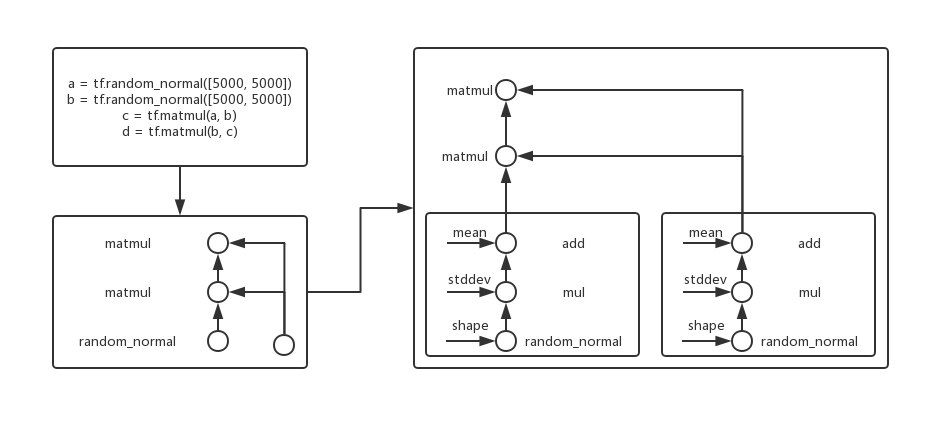
\includegraphics[width=0.8\textwidth]{figures/dag_mat.jpg}
        \caption{数据流图的创建过程}
        \label{fig:dag_mat}
    \end{figure}

    {\bfseries 图的传送} 将数据流图序列化并发送。用户创建的会话并不直接执行数据流图的计算,而是将图先发送给主机(master),主机再将任务划分发送给从机(worker)去执行。这一步,先将数据流图转化为一种易于传输的形式,再进行发送。
    
    {\bfseries 图的剪枝} 求图的最小依赖集。这一步在主机上进行,首先将得到的序列转化为数据流图。根据之前给定的输入输出列表,对图进行剪枝,删除不需要被执行的节点。在TensorFlow的实现中,这一步使用深度优先搜索进行。

    {\bfseries 图的划分} 将图分配到不同从机。 在TensorFlow中进行多机并行的时候,需要手动对计算指定运行的从机。这部分的工作就是根据用户的指定,将图切分,并传输到相应的从机上。

    {\bfseries 图的二次划分} 将图分配到不同设备。这一步在从机上进行。TensorFlow会根据当前可用的设备,和用户对操作指定的设备,将图再次切分,将各部分分配到不同设备上,默认情况下,TensorFlow会把操作尽量分给GPU。在单机多GPU的情况下,用户需要手动指定操作执行的GPU编号。
    
    {\bfseries 图的运行} 运行子图。从机为每个子图创建一个执行器对象,用来运行这个子图。经过两次划分,现有的子图可以直接在同一个设备上执行。执行器等待依赖的数据,数据准备完毕后直接执行。执行器就是Stream Executor的实例,对操作进行封装。
    
    调度模拟部分主要工作就是执行以上流程,从图的创建开始,到两次划分为止,图的运行被替换成了调用性能模型。我们的实验主要在单机上进行,因此图的传送和第一次划分在我们的系统中没有相应的实现。
